%# -*- coding:utf-8 -*-
\documentclass[10pt,aspectratio=169,mathserif]{beamer}		
%设置为 Beamer 文档类型,设置字体为 10pt,长宽比为16:9,数学字体为 serif 风格

%%%%-----导入宏包-----%%%%
\usepackage{zju}			%导入 zju 模板宏包
\usepackage{ctex}			%导入 ctex 宏包,添加中文支持
\usepackage{amsmath,amsfonts,amssymb,bm}   %导入数学公式所需宏包
\usepackage{color}			 %字体颜色支持
\usepackage{graphicx,hyperref,url}
\usepackage{metalogo}	% 非必须
\usepackage{ragged2e}

\usepackage{tikz}

%%绘图用的宏包
\usepackage{pgfplots}
\pgfplotsset{compat=newest}
%% 上文引用的包可按实际情况自行增删
%%%%%%%%%%%%%%%%%%
\usepackage{fontspec}
\usepackage{xeCJK}
% \setCJKmainfont{Source Han Sans SC}



\beamertemplateballitem		%设置 Beamer 主题

%%%%------------------------%%%%%
\catcode`\。=\active         %或者=13
\newcommand{。}{.}				
%将正文中的“。”号转换为“.”。中文标点国家规范建议科技文献中的句号用圆点替代
%%%%%%%%%%%%%%%%%%%%%

%%%%----首页信息设置----%%%%
\title[遗传算法的数学理论和欺骗问题]{遗传算法的数学理论和欺骗问题}
\subtitle{--模式定理和欺骗问题}			
%%%%----标题设置


\author[罗俊勋]{
  罗俊勋
}
  
\institute[IOPP]{
  School of Mathmatical\\ 
  Zhejiang University}
%%%%----机构信息

\date[Sept. 25 2024]{
  2024年9月25日}
%%%%----日期信息
  
\begin{document}

\begin{frame}
	\titlepage
\end{frame}				%生成标题页


\begin{frame}
%%  	\frametitle{提纲}
	\tableofcontents
\end{frame}				%生成提纲页


\section{引言}
\begin{frame}
	\frametitle{引言}
  
  \begin{block}{Problem}
      求函数最大值
      $$f(x, y) = \sqrt{8 - x^2 - y^2} + 1, \quad (x, y) \in [-2, 2] \times [-2, 2]$$
  \end{block}

    \begin{columns} % 开始两列布局
        \begin{column}{0.6\textwidth} % 左侧列占据 60% 宽度
            \begin{itemize}
              \item 编码方式: $x=a_0.a_1a_2a_3, y=b_0.b_1b_2b_3 \rightarrow a_0a_1a_2a_3b_0b_1b_2b_3$
              \begin{itemize}
                \item 如:$x=1.213, y=0.872 \rightarrow 12130872$
              \end{itemize}

              \item 考虑形如 $abcd****$ 的编码,这对应了一个解空间的子集 $\{(a.bcd,y)|y\in [-2,2]\}$

                \begin{itemize}
                  \item $0000****$ 为最优的(在平均适应度意义下)
                  \item 包含最优解
                \end{itemize}

            \end{itemize}
        \end{column}

        \begin{column}{0.4\textwidth} % 右侧列占据 40% 宽度
            \begin{flushright}
                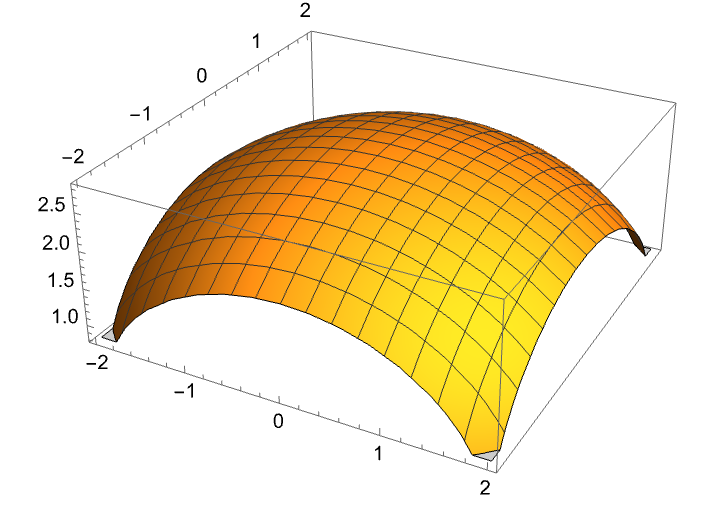
\includegraphics[width=\textwidth]{img/f.png} % 设置图片宽度适应列宽
            \end{flushright}
        \end{column}
    \end{columns}
\end{frame}


\section{模式定理}


\begin{frame}
  \frametitle{符号说明}
  \begin{block}{定义}

  以下的讨论都是基于基本遗传算法(SGA)的模型,即二进制编码,单点交叉,单点变异,比例选择

    \begin{itemize}
      \item 模式: 表示一些相似的模块,描述了在某些位置上具有相似结构特征的个体编码串的一个子集

      \begin{itemize}
        \item $H=1*0*1 = \{10001,11001,10011,11011\}$
        \item 在含有 $k$ 个基本字符的字母表上长度为 $l$ 的字符串中的模式共有 $(k+1)^l$ 个
      \end{itemize}

      \item 模式阶($\text{Schema Order}$): $o(H)$ 表示模式 $H$ 中具有确定基因值的位置的数目 
      \begin{itemize}
        \item 例如: $o(1*0*1)=3$
      \end{itemize}

      \item 模式定义长度($\text{Schema Length}$): $\delta(H)$ 表示模式 $H$ 第一个和最后一个确定基因值之间的距离
      \begin{itemize}
        \item 例如: $\delta(1*0*1)=4$
        \item 定义: $\delta(**1*) = 1$ (为什么不是0)
      \end{itemize}
  
      \item $P(t):$ 第 $t$ 代群体, $F$ 适应度函数, $A_i$ 个体, 种群大小 $M$
      \item $m(H,t):$ 第 $t$ 代群体中与模式 $H$ 匹配的个数

    \end{itemize}

  \end{block}
\end{frame}

\begin{frame}
  \frametitle{选择算子}
  \begin{block}{选择算子的作用}
    第 $t$ 代群体的总适应度为$F(t) =\sum\limits_{i} F(A_i)$, 平均适应度为 $\bar{F}(t) = \frac{F(t)}{M}$

    个体$A_i$ 平均复制了 $M\frac{F(A_i)}{F(t)}$ 个后代, 设与 $H$ 匹配的个体的平均适应度为 $f(H,t)$


    \begin{align*}
      m(H,t+1) &= \sum\limits_{A_i\in H\cap P(t)} \frac{M\cdot F(A_i)}{F(t)} \\
               &=  \frac{M}{F(t)}  \sum\limits_{A_i\in H\cap P(t)} F(A_i) \\
               &=  \frac{1}{\bar{F}(t)} f(H,t) \times \#\{A_i\in H\cap P(t)\} \\
               &= m(H,t) \times \frac{f(H,t)}{\bar{F}(t)}
    \end{align*}
  \end{block}
\end{frame}

\begin{frame}
  \frametitle{选择算子}

  \begin{block}{选择算子的作用}
    最终得到递推式 
    
  $$m(H,t+1) = m(H,t) \times \frac{f(H,t)}{\bar{F}(t)}$$

    可以看出, 如果这个模式的平均适应度是偏高的,那么在下一代中, 符合这个模式的个体数目会增加
    
    进一步,假设模式 $H$ 的平均适应度总是高出群体平均适应度的 $C$ 倍, 那么上式可记为

  $$m(H,t+1)=(1+C)m(H,t)$$

    于是,如果 $C>0$, 则 $m(H,t)$ 呈指数级增长, 若 $C<0$ 则指数级衰减
  \end{block}


 \begin{block}{结论}
  选择算子使得高适应度模式的个体数目指数增长, 低适应度模式的个体数目指数减少
 \end{block} 
\end{frame}



\begin{frame}
  \frametitle{交叉算子}

  \begin{block}{交叉算子的作用}
  
    \begin{figure}
      \begin{center}
        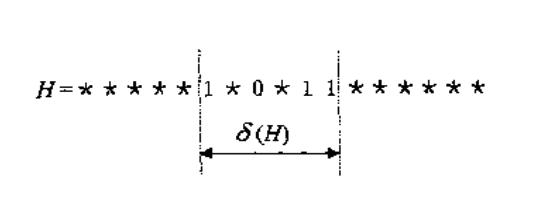
\includegraphics[width=0.4\textwidth]{img/H.jpg}
      \end{center}
    \end{figure}

    只有当设置的交叉点在模式的定义长度之内,交叉操作才有可能破换模式

    这样模式在一次交叉操作中生存的下界为

    $$p_{surcvival} = 1 - p_c\frac{\delta(H)}{l-1}$$

    于是经过选择和交叉操作后,模式的样本数满足

    $$m(H,t+1)\geq m(H,t)\cdot ( 1+C )\cdot \left[1 - p_c\frac{\delta(H)}{l-1} \right]$$

  \end{block}
\end{frame}


\begin{frame}
  \frametitle{变异算子}

  \begin{block}{变异算子的作用}
    如变异使得某一模式被破坏,那么变异的点位必定是模式描述形式中通配符 "*" 之外的某一基因值发生变化,其概率为

    $$1- (1-p_m)^{o(H)}$$

    因为 $p_m$ 非常接近于 0, 于是有

    $$1- (1-p_m)^{o(H)} \approx p_m \cdot o(H)$$

    因此模式生存的概率为

    $$1-p_m \cdot o(H)$$

  \end{block}

\end{frame}


\begin{frame}
  \frametitle{模式定理}
  
  \begin{block}{ }
    综合上面的式子, 忽略一些极小项,可以得到

    $$m(H,t+1) \geq m(H,t) \cdot (1+C) \cdot \left[1 - p_c\frac{\delta(H)}{l-1} -p_m \cdot o(H) \right]$$

    这就得到以下定理

    \begin{block}{模式定理}
      遗传算法中,在选择、交叉和变异算子的作用下,具有低阶、短的定义长度,并且平均适应度高于群体平均适应度的模式将按指数级增长
    \end{block}
  \end{block}

\end{frame}


\section{积木块假设和遗传算法的欺骗问题}

\begin{frame}
  \frametitle{积木块假设}

  \begin{block}{积木块}
    模式定理中所指的具有低阶、短定义长度以及平均适应度高于种群平均适应度的模式被定义为积木块( Building Block)
  \end{block}

  \begin{block}{积木块假设}
  遗传算法通过短定义距、低阶以及高于平均适应度的模式(积木块),在遗传操作作用下相互结合,最终接近全局最优解
  \end{block}
  
\end{frame}

\begin{frame}
  \frametitle{欺骗问题}

  求函数 $f(x, y)$ 的最大值:

  \[
  f(x, y) = 
    \begin{cases} 
      -\sqrt{8 - x^2 - y^2} + 1 & (x, y) \in [-2, 2] \times [-2, 2] \setminus \{(0,0)\} \\ 
      100 & (x, y) = (0,0) 
    \end{cases}
  \]

  \begin{figure}
    \centering
    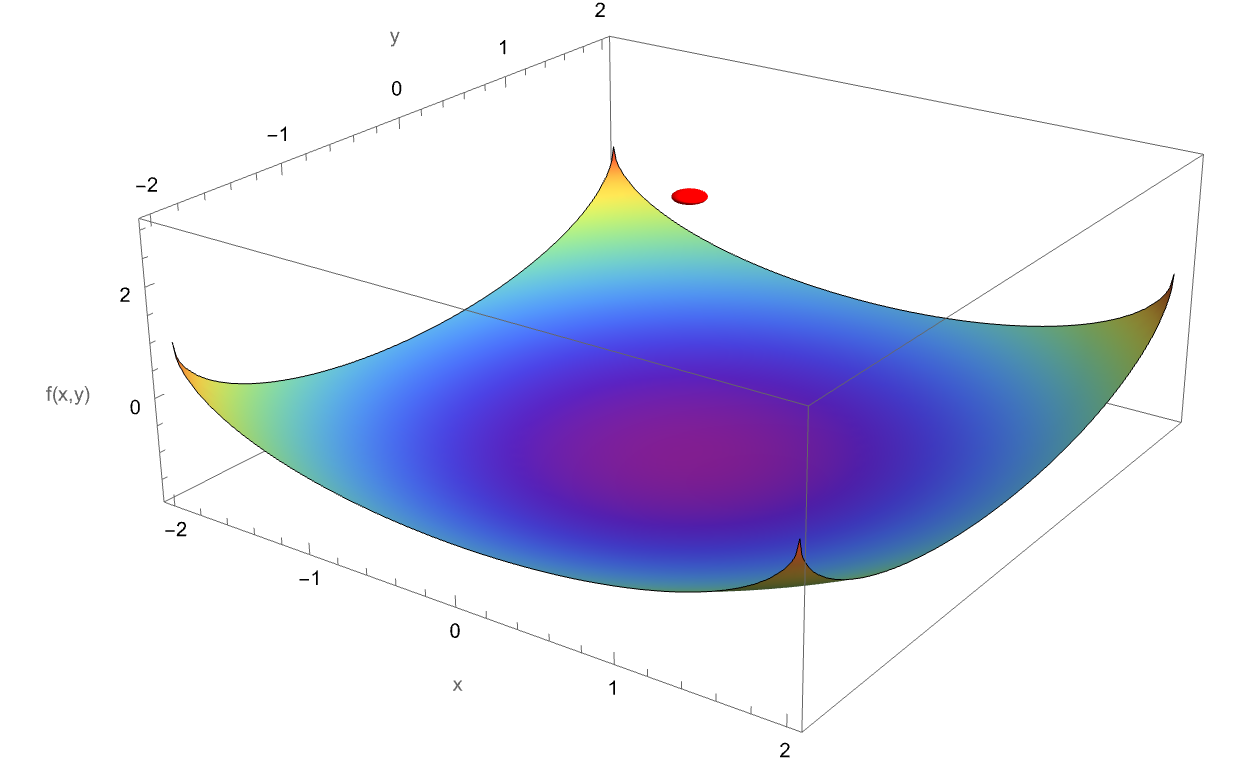
\includegraphics[width=0.4\textwidth]{img/H1.png}
    \caption{ $f(x, y)$ 图示}
  \end{figure}

\end{frame}



\begin{frame}
  \frametitle{欺骗问题}
  \begin{block}{定义}
妨碍评价值高的个体生成从而影响遗传算法正常工作的问题统称为欺骗问题
  \end{block}

  \begin{block}{竞争模式}
    若在模式 $H$ 和 $H^\prime$ 中, $*$ 的位置完全一致,但是任一确定位的编码均不一样, 则称 $H$ 和 $H^\prime$ 互为竞争模式 ; 如 $H=0*0*1, H^\prime=1*1*0$
  \end{block}

  \begin{block}{欺骗问题的类型}
考虑一个 2 位二进制最大化问题, 假定 "11"对应最优解, 若 $H(0 *)>H(1 *)$, 则欺骗性存在,即为 $\frac{f(00)+f(01)}{2}>\frac{f(10)+f(11)}{2}$

设 $r=f(11) / f(00), c=f(01) / f(00), c^{\prime}=f(10) / f(00)$, 那么上式化为
$$
r<1+c-c^{\prime}
$$

将 $c>1$ 的情况称为 I 类欺骗问题, $c \leqslant 1$ 的情况称为 II 类欺骗问题
  \end{block}

\end{frame}

\begin{frame}
  \frametitle{欺骗问题的化解}
  \framesubtitle{以最小化举例}

  \begin{itemize}
    \item 1. 调整编码:
  \end{itemize}

  \begin{columns}
    % 左侧的表格
    \begin{column}{0.5\textwidth} 
      \begin{table} 
        \centering
        \caption{二进制编码函数值}
        \begin{tabular}{c|c|c}
        \hline 编码 & 对应整数解 & 函数值 \\
        \hline 00 & 0 & 4 \\
        01 & 1 & 3 \\
        10 & 2 & 1 \\
          11 & {\color{red}3} & 5 \\
        \hline
        \end{tabular}
      \end{table}
    \end{column}

    % 右侧的表格
    \begin{column}{0.5\textwidth} 
      \begin{table} 
        \centering
        \caption{Grey 编码函数值}
        \begin{tabular}{c|c|c}
        \hline 编码 & 对应整数解 & 函数值 \\
        \hline 00 & 0 & 4 \\
        01 & 1 & 3 \\
        11 & 2 & 1 \\
          10 & {\color{red}3} & 5 \\
        \hline
        \end{tabular}
      \end{table}
    \end{column}
  \end{columns}

  \begin{itemize}
    \item 2. 调整适应度函数:
  \end{itemize}

  设目标函数 $g(00)=128, g(01)=1, g(10)=g(11)=32$, 如果适应度函数 $f(x)=g(x)$, 则 $f(0*)=64.5, f(1*)=32$,因此存在欺骗问题。

  如果用适应度函数的调整方法, $f(x)=\log_2 g(x)$, 则$f(00)=7, f(01)=0, f(11)=f(10)=5$

  从而得到 $f(0*)=3.5, f(1*)=5$,这就避免了欺骗问题的产生。

\end{frame}



\section{GA-hard问题}

\begin{frame}
  \frametitle{遗传算法难解问题}
  \begin{block}{定义}
    将采用基本的遗传操作包括选择和再生、交叉与变异,以及标准的操作参数,进行模拟进化的过程求解最优解很容易的场合,称为遗传算法的容易问题;反之,称为遗传算法的困难问题。

    欺骗问题和遗传算法困难问题不等价
  \end{block}

  \begin{itemize}
    \item 复杂目标函数:目标函数不光滑或具有多个局部最优解。
    \item 高维度:搜索空间维度较高,搜索空间大。
    \item 约束性:问题可能有很多约束,限制了解的搜索空间。
  \end{itemize}
\end{frame}

\end{document}
